\documentclass[a4paper,12pt]{article}
\usepackage{bbding,combelow,textcomp,amsfonts,amsthm,amsmath,amssymb,graphicx,color,hyperref,etoolbox}
\usepackage[utf8x]{inputenc}
\usepackage[lined,boxed,commentsnumbered]{algorithm2e}

\newtoggle{story}


%%%%%%%%%%%%%%%%%%%%%%%%%%%%%%%%%%%%%%%%%%
%% Customisation options --- update as necessary
%%%%%%%%%%%%%%%%%%%%%%%%%%%%%%%%%%%%%%%%%%

%% Course details: title, semester, instructors

\newcommand{\courseTitle}{Combinatorics II (Math 7702)}
\newcommand{\semester}{Spring 2026}
\newcommand{\instructorA}{Shagnik Das}
\newcommand{\instructorB}{Lu Yun-Chi}

%% Sheet number

\newcommand{\sheetNumber}{5}


%% Submission details

\newcommand{\dueDate}{12:20, Jun 5th.}
\newcommand{\lateWarning}{Late submissions will receive no credit.}


%% Display irrelevant footnotes?  \toggletrue for yes, \togglefalse for no

\toggletrue{story}

%%%%%%%%%%%%%%%%%%%%%%%%%%%%%%%%%%%%%%%%%%
%% End of customisation options
%%%%%%%%%%%%%%%%%%%%%%%%%%%%%%%%%%%%%%%%%%

\pdfpagewidth 8.5in
\pdfpageheight 11in
\topmargin -1in
\headheight 0in
\headsep 0in
\textheight 8.5in
\textwidth 6.5in
\oddsidemargin 0in
\evensidemargin 0in
\headheight 77pt
\headsep 0in
\footskip .75in

\makeatletter
\newcommand{\buildtitle}[4]{
\begin{flushleft}
{\large
#1
\hfill{}
#2
\par
#3
}
\end{flushleft}
\vskip 4pt
\begin{center}
{\large\bfseries#4\par}
\end{center}
\bigskip
}
\makeatother

\renewcommand{\thesection}{\normalsize\arabic{section}}

\renewcommand{\deg}{\textrm{deg}}
\newcommand{\eps}{\varepsilon}
\newcommand{\ceil}[1]{\left \lceil #1 \right \rceil}

\newcommand{\hint}{\begin{flushright} [Hint at \url{\hintURL}.] \end{flushright}}

\newcommand{\card}[1]{\left| #1 \right|}
\newcommand{\mb}[1]{\mathbb{#1}}
\newcommand{\mc}[1]{\mathcal{#1}}
\newcommand{\chil}{\chi_{\ell}}


\newcommand{\story}[1]{\iftoggle{story}{\footnote{#1}}{}}
\newcommand{\storymark}[1][42]{\iftoggle{story}{\footnotemark[#1]}{}}
\newcommand{\storytext}[2][42]{\iftoggle{story}{\footnotetext[#1]{#2}}{}}

\newcommand{\bonus}[2]{\paragraph{Bonus (#1 pt\ifstrequal{#1}{1}{}{s})} #2}


\begin{document}


\buildtitle{\courseTitle{}}{\semester}{\instructorA{} \hfill \instructorB{}}{Exercise Sheet \sheetNumber{}}

\vspace{-0.2in}

\begin{center}

{B13902024 Chang, Yi-Kuei \\ \bf Due date: \dueDate \\ \lateWarning}

\end{center}

\noindent You should try to solve all of the exercises below, and then submit two solutions to be graded --- each problem is worth $10$ points. Make sure to clearly justify your answers, defining everything precisely and stating any results you are using. You should then submit your solutions on NTU COOL, either as a typed PDF or a clear picture or scan of your handwritten answers.

\paragraph{Exercise 1}  Show that the complete $k$-partite graph $K_{\underbrace{2,2,\hdots,2}_{k \textrm{ parts}}}$ with $k$ parts each of size two has $\chil(K_{2,2,\hdots,2}) = k$.

\paragraph{Solution:}

Let $G_k = K_{\underbrace{2,2,\hdots,2}_{k \text{ parts} }}$ with parts $V_i = \{x_i, y_i\}$ for $i = 1, \ldots, k$.

\medskip
\noindent\textbf{Step 1: $\chil(G_k) \geq k$.}

Since $\chil(G_k) \geq \chi(G_k) \geq \omega(G_k)$, and $\{x_1, x_2, \ldots, x_k\}$ is a clique in $G_k$, we have $\omega(G_k) \geq k$, hence $\chil(G_k) \geq k$.

\medskip
\noindent\textbf{Step 2: $\chil(G_k) \leq k$.}

We proceed by induction on $k$.

\textit{Base case:} $k = 1$, then $G_1 = (V, \emptyset)$, so trivially $\chil(G_1) \leq 1$.

\textit{Inductive step:} Assume the statement holds for $k-1$. Consider an arbitrary list assignment $\{L_v\}_{v \in V(G_k)}$ with $\card{L_v} = k$ for all $v \in V(G_k)$.

\textbf{Case 1:} $\exists\, i$ such that $L_{x_i} \cap L_{y_i} \neq \emptyset$.

Pick a color $c \in L_{x_i} \cap L_{y_i}$ and assign it to $x_i$ and $y_i$. Remove $c$ from every list $L_v$ (for $v \in V(G_k)$) whenever $c \in L_v$. Then $G_k - \{x_i, y_i\} \cong G_{k-1}$, and by the induction hypothesis we can properly list-color $G_{k-1}$ since all remaining lists have size $\geq k - 1$. Restoring the vertices $x_i, y_i$ with color $c$ yields a proper list-coloring of $G_k$ using $\{L_v\}_{v \in V(G_k)}$.

\textbf{Case 2:} $\forall\, i$, $L_{x_i} \cap L_{y_i} = \emptyset$.

Construct a bipartite graph $B = (X \cup Y, E)$ where $X = V(G_k)$, $Y = \bigcup_{x \in V(G_k)} L_x$, and $\{x, y\} \in E(B)$ for $x \in X$, $y \in Y$ if and only if $y \in L_x$. A perfect matching in $B$ assigns each vertex of $G_k$ a distinct color from its list; since all vertices receive different colors, any two adjacent vertices (which lie in distinct parts) are colored differently, giving a proper list-coloring.

We verify Hall's condition: for all $W \subseteq X$,
\[
\left|\bigcup_{v \in W} L_v\right| \geq \card{W}.
\]

\textit{Subcase 1:} $\card{W} \leq k$. Since $\card{L_v} = k$ for every $v \in W$, picking any $v_0 \in W$ gives $\left|\bigcup_{v \in W} L_v\right| \geq \card{L_{v_0}} = k \geq \card{W}$.

\textit{Subcase 2:} $\card{W} > k$. Since $G_k$ has only $k$ parts, by the pigeonhole principle there exists $j$ such that $x_j, y_j \in W$. Since $L_{x_j} \cap L_{y_j} = \emptyset$, we have $\card{L_{x_j} \cup L_{y_j}} = 2k$. Since $W \subseteq X = V(G_k)$, we have $\card{W} \leq \card{V(G_k)} = 2k$. Therefore,
\[
\left|\bigcup_{v \in W} L_v\right| \geq \card{L_{x_j} \cup L_{y_j}} = 2k = \card{V(G_k)} \geq \card{W}.
\]

Hall's condition holds, so a perfect matching in $B$ exists, completing the proof. \hfill$\square$

\paragraph{Exercise 2}  Prove that any bipartite graph $G$ with non-empty lists $L = \{L(v) : v \in V(G) \}$ satisfying $\card{L(u) \cap L(v)} \neq 1$ for every edge $\{u,v\} \in E(G)$ has a proper $L$-colouring.

\paragraph{Solution:}

Suppose $G = (A \cup B, E)$. Let $C = \bigcup_{v \in V(G)} L(v)$.

Since each $L(v)$ is finite, the set $C$ is finite, so we can impose a strict total order $<$ on $C$ by labeling each color with a unique number and comparing colors by their labels.

Define a coloring $c \colon A \cup B \to C$ by
\begin{itemize}
    \item $c(u) = \min(L(u))$ \quad for all $u \in A$,
    \item $c(v) = \max(L(v))$ \quad for all $v \in B$.
\end{itemize}

We claim $c$ is a proper $L$-colouring. Suppose not; then there exist $u \in A$, $v \in B$ with $\{u, v\} \in E(G)$ and $c(u) = c(v)$, i.e.\ $\min(L(u)) = \max(L(v))$.

Hence for every $c_1 \in L(u) \setminus \{\min(L(u))\}$ and $c_2 \in L(v) \setminus \{\max(L(v))\}$ we have $c_1 > c_2$, so the only element that can belong to both $L(u)$ and $L(v)$ is $\min(L(u)) = \max(L(v))$. Therefore
\[
\card{L(u) \cap L(v)} = \card{\{\min(L(u))\}} = \card{\{\max(L(v))\}} = 1,
\]
contradicting the hypothesis. \hfill$\square$

\paragraph{Exercise 3}  Let $G$ be a graph with maximum degree $\Delta = \Delta(G)$.
\begin{itemize}
	\item[(a)] Show that if the vertices in $G$ of degree $\Delta$ induce a forest (that is, a graph without cycles), then $G$ is $\Delta$-edge-colourable.
	\item[(b)] Show that for every matching $M$ in $G$, there is a $(\Delta + 1)$-edge-colouring of $G$ in which all edges of $M$ receive the same colour.
\end{itemize}

\paragraph{Exercise 4}  Your mission, should you choose to accept it, is to extend the proof of Galvin's theorem from $K_{n,n}$ to general bipartite graphs.
\begin{itemize}
	\item[(a)] Let $G$ be a bipartite graph with edge-chromatic number $\chi'(G) = n$. Adapting the ideas behind the orientation of $L(K_{n,n})$ from lectures, use an $n$-colouring of $E(G)$ to find an orientation $\vec{D}$ of the line graph $L(G)$ such that:
	\begin{itemize}
		\item[(i)] The maximum out-degree is at most $n-1$.
		\item[(ii)] Given an edge $\{x,y\}$ of $G$, the digraphs induced on the sets $S_x = \{ \{x,y'\} : y' \in N(x) \} \subset V(L(G))$ and $S_y = \{ \{x', y \} : x' \in N(y) \} \subset V(L(G))$ are transitive.
	\end{itemize}
	\item[(b)] Show that $\vec{D}$ is kernel-perfect, and deduce that $\chi'_{\ell}(G) = n$.
\end{itemize}


\paragraph{Exercise 5}  In this exercise we will prove that Thomassen's theorem is tight; that is, there are planar graphs that are not $4$-choosable.
\begin{itemize}
	\item[(a)] Show that the following graph has no proper coloring from the assigned lists.
(In this part of the exercise, $\bar{i}$ denotes the set $[4]\setminus \{ i\}$.)
\begin{center}
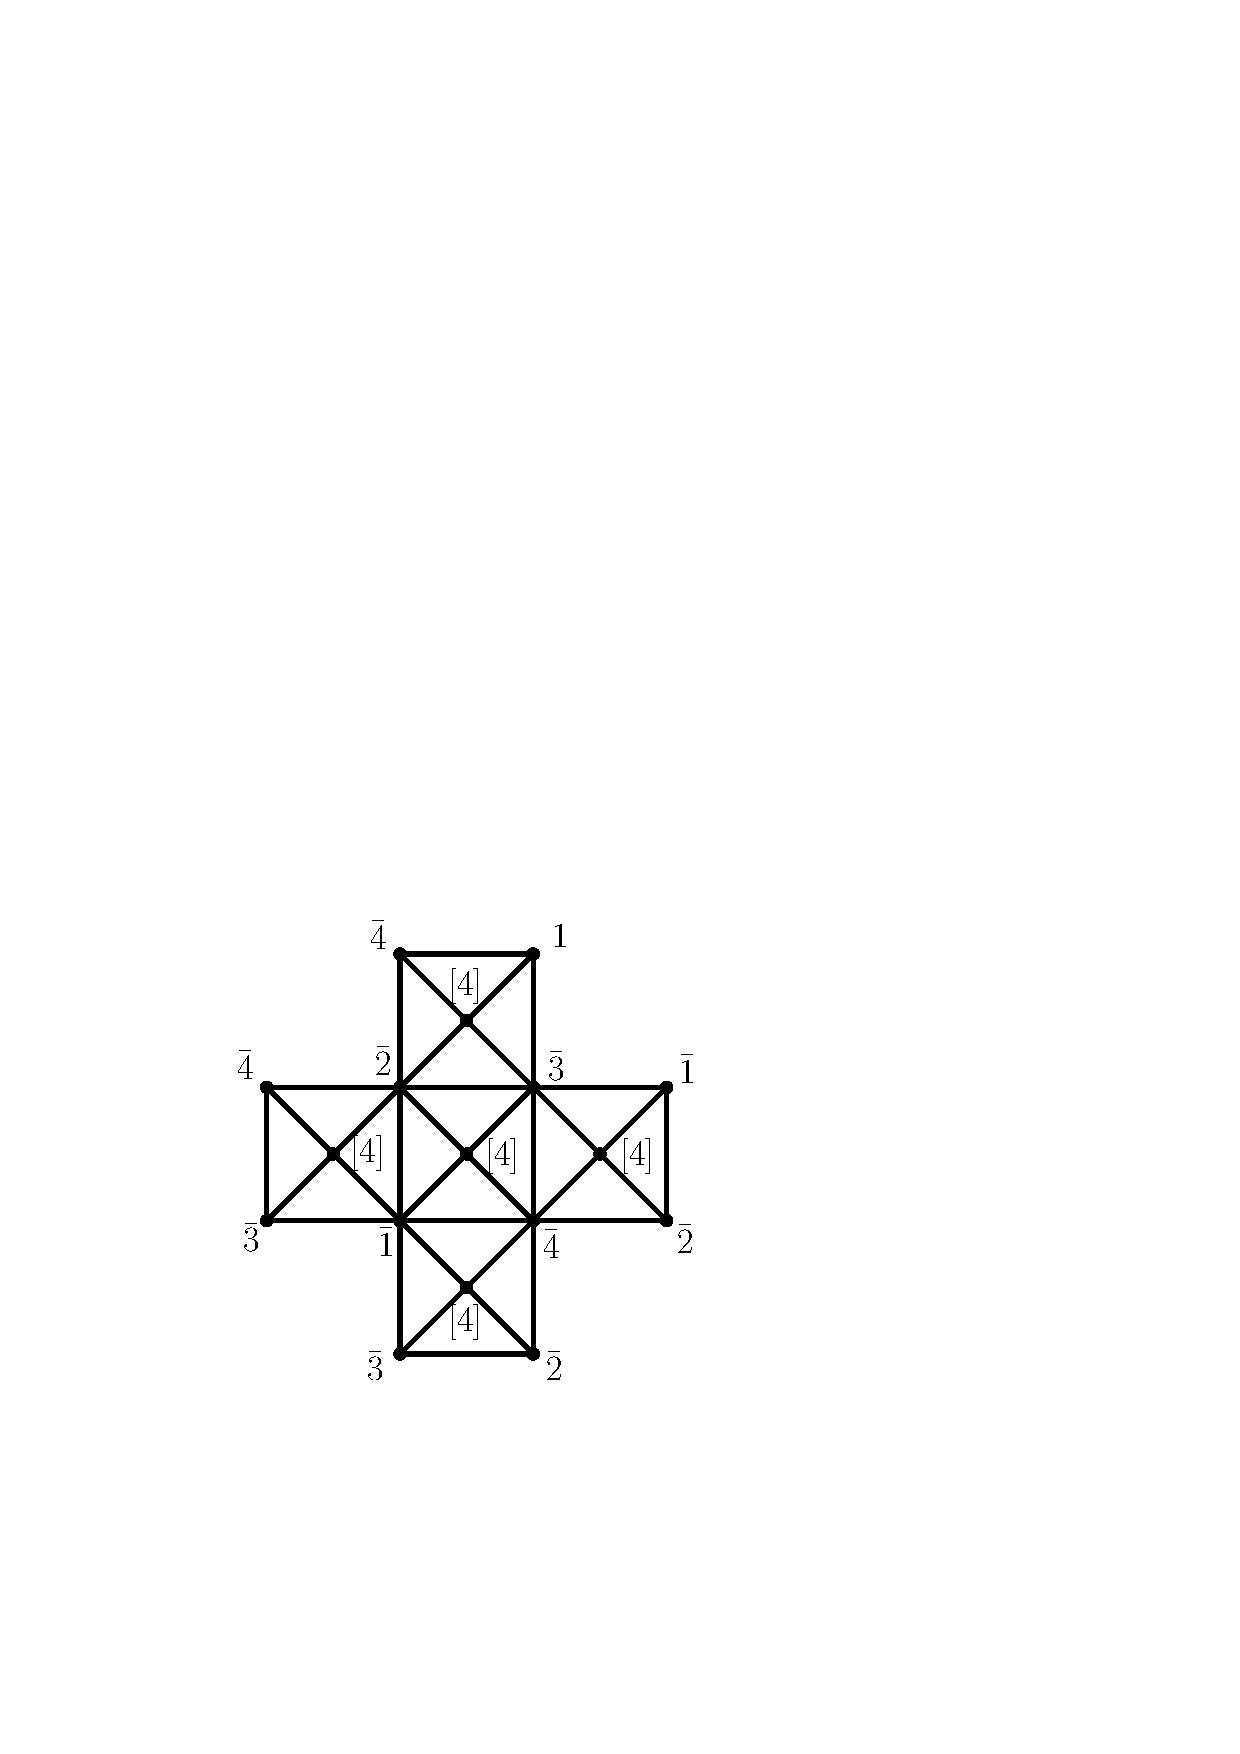
\includegraphics[width=5cm]{sheet5pic1.pdf}
\end{center}
	\item[(b)] Let $G$ be the graph obtained from the graph below by adding an extra vertex to the outside face and connecting it to all the vertices on the boundary. Show that if the new vertex is assigned the list $\bar{1}$, then there is no proper list coloring of $G$ from the assigned lists.
(In this part of the exercise, $\bar{i}$ denotes the set $[5]\setminus \{ i\}$.)
\begin{center}
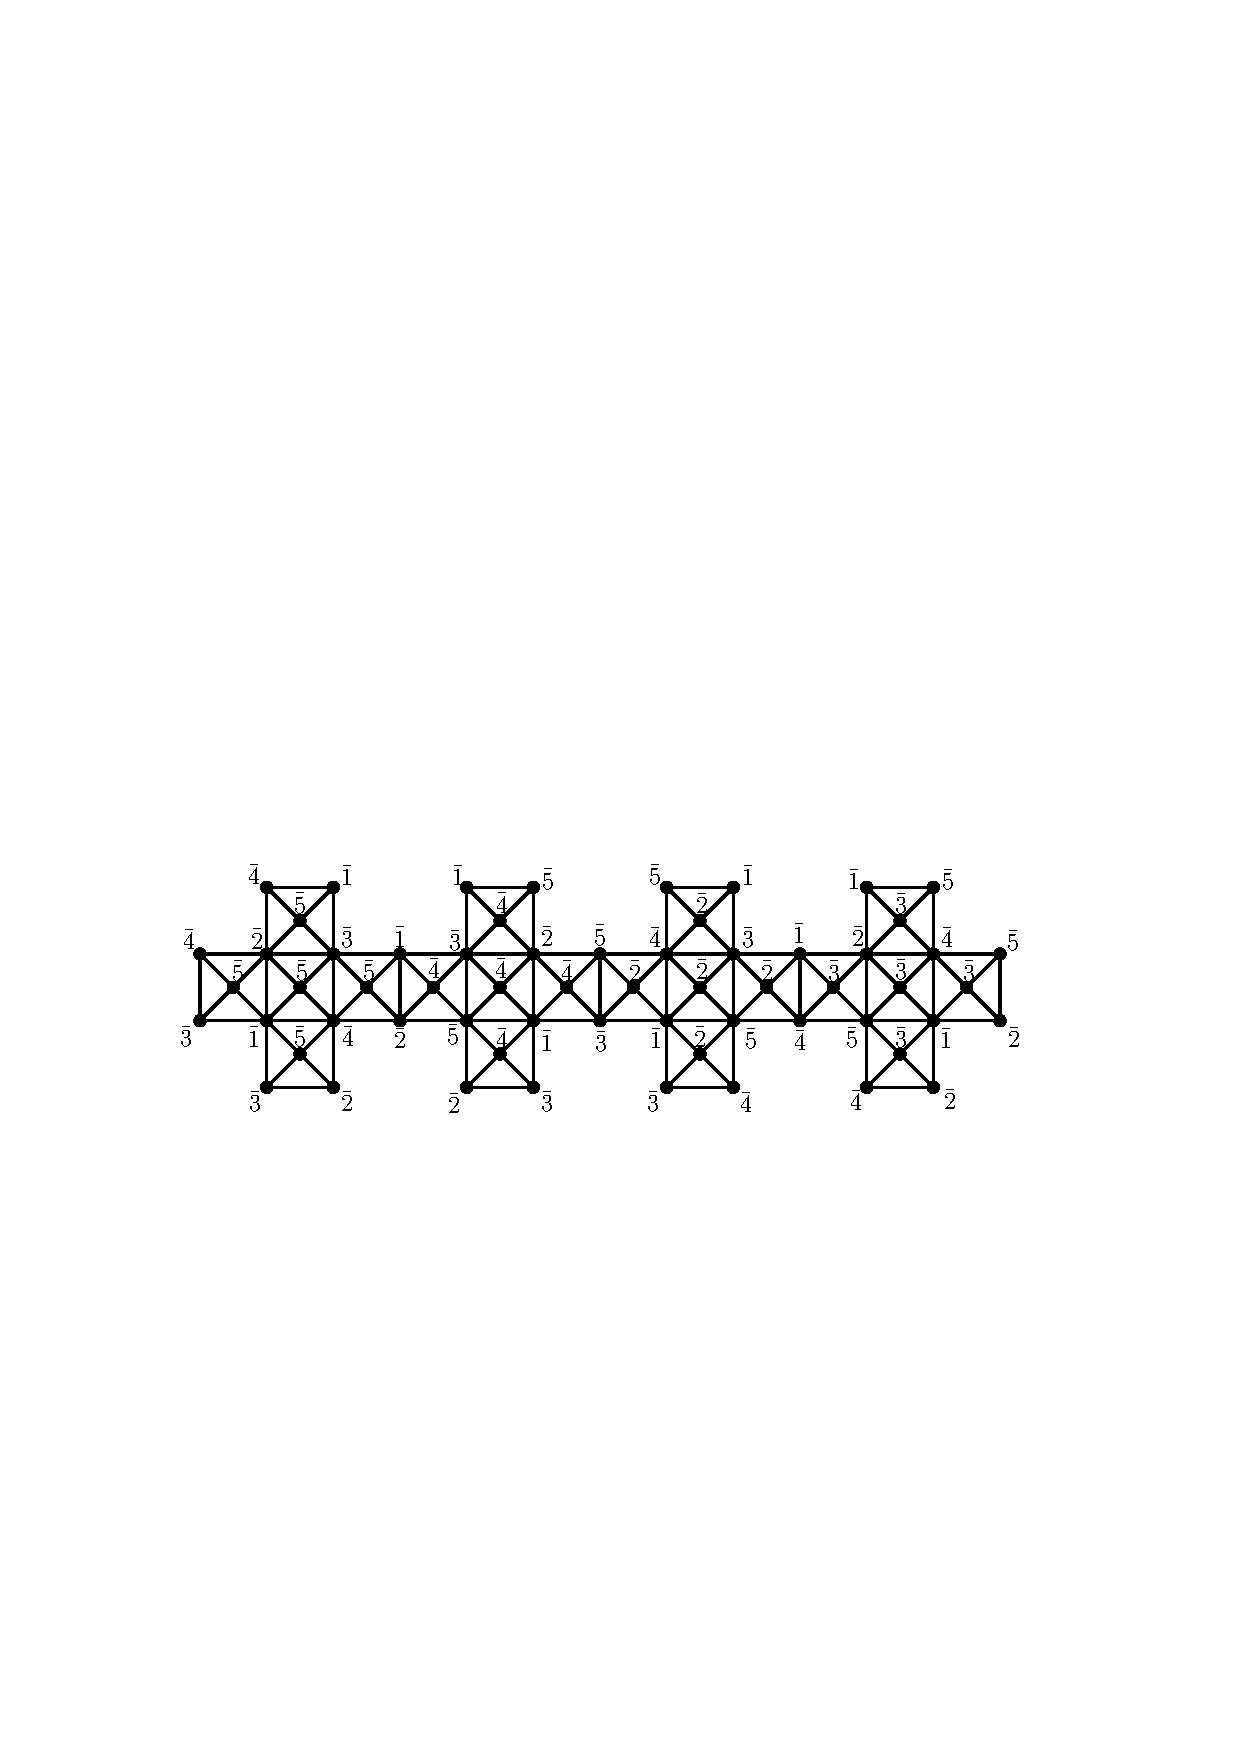
\includegraphics[width=14cm]{sheet5pic2.pdf}
\end{center}
\end{itemize}

% \newpage

% \section*{Hints}  The following QR codes contain hints for some of the homework exercises.  You should be able to decode them using any QR code scanner, including this one: \url{https://zxing.org/w/decode.jspx}.

% \paragraph{Exercise ?} Also available at \url{https://i.ibb.co/???????/S??E?.png}.

\begin{center}
% \includegraphics[scale=0.5]{Hints/S??E?.png}
\end{center}

\end{document}